\documentclass[11pt]{scrartcl}
\usepackage[utf8]{inputenc}
\usepackage{evank}


%% insert title here
\newcommand{\titlee}{Conductors}
\parindent 0 pt

\newcommand{\officialsol}[1]{See the official solutions \href{#1}{here}.}

\title{\titlee}
\author{Cambridge Physics Academy}
\date{2023-2024}


\begin{document}

\thispagestyle{empty}
\begin{center}
    
    
    \Huge \textbf{\textsf{\titlee}}

    \large \theauthor
\end{center}

\setcounter{section}{-1}
\section{Readings}
\begin{itemize}
    \item HRK Chapters 29-30
    \item Purcell Chapter 3
\end{itemize}
Feel free to do problems from the readings as extra practice.


\section{Lecture review}

\begin{defn}[Electric Potential]
    The electric potential $\phi$ is a scalar quantity reflecting the potential energy per unit charge of a point in space. The potential difference (sometimes called \textit{voltage}) between two points $P_1$ and $P_2$ is related to electric field via $$\Delta \phi=-\int_{P_1}^{P_2}\mathbf E\cdot d\mathbf r$$Consequently the electric field is related to the potential via $$\mathbf E=\left(-\frac{d\phi}{dx},-\frac{d\phi}{dy},-\frac{d\phi}{dz}\right)\equiv -\nabla\phi$$ If we set potential to be 0 at infinity, then the potential at at a given point is well defined: $$\phi=-\int_\infty ^{P}\mathbf E\cdot d\mathbf r$$We can also find the potential at a given point from integrating the scalar contributions from charge in space: $$\phi=\int_V\frac{\rho}{4\pi\epsilon_0 r}dv$$
    Given some charge configuration with potential $\phi$ defined at every point in space, moving a charge $q$ from one point to another changes its potential energy via the change in potential: $$\Delta U=q\cdot\Delta \phi$$
\end{defn}

\begin{defn}[Potential Energy]
    The potential energy of a charge distribution can be found in two ways. The first, using the electric potential $\phi$ and charge $\rho \, dv$ at all points in space, $$U=\frac 12\int_V\phi \rho \, dv$$The factor $1/2$ comes from the fact that the integral counts each pairwise charge interaction twice, so we divide by 2 to avoid overcounting. The second method is to integrate the potential energy density, which is defined as $$\mathcal U=\frac12\epsilon_0 E^2$$ which is the energy associated with the presence of an electric field $E$ at a given point in space. As a result, the other form of $U$ is $$U=\int_V\mathcal U \, dv=\frac12\epsilon_0\int_V E^2\, dv$$
\end{defn}
\begin{defn}[Conductors]
Conductors are materials in which electrons are free to move. When a conductor is placed into an external electric field, the electrons will move into a configuration at which they stop moving, i.e. when no electric field acts on them anymore. Thus, \textbf{a conductor has zero electric field inside it.} Some other properties of conductors include \begin{itemize}
    \item $\phi$ is a constant value throughout the conductor.
    \item all charge on a conductor is distributed on its surface.
    \item the electric field lines right outside a conductor are directed perpendicular to the surface of the conductor and has strength $E=\sigma/\epsilon_0$. 
\end{itemize}
\end{defn}

\begin{theorem}[Image Charges]
    Given a charge in the vicinity of a conductor, the charge on the surface conductor will redistribute itself so that the external electric field is directed perpendicularly to the conductor. This redistributed charge will induce a force on the original. There are two special cases of image charges to take note of: \begin{itemize}
        \item An infinite conducting plane: For a charge $q$ placed above the plane, the electric field is distributed as if there were an opposite charge $-q$ on the mirror side of the plane. 
        \begin{center} 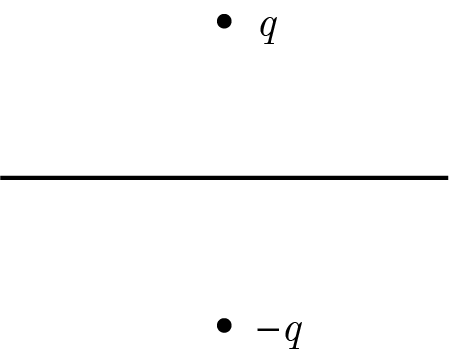
\includegraphics[scale=1]{plane} \end{center}
        \item A spherical conducting shell: For a charge $q$ placed a distance $r$ from the center of the shell of radius $R$, the electric field is distributed as if there were an opposite charge $-qR/r$ a distance $R^2/r$ from the center of the shell. 
        \begin{center} 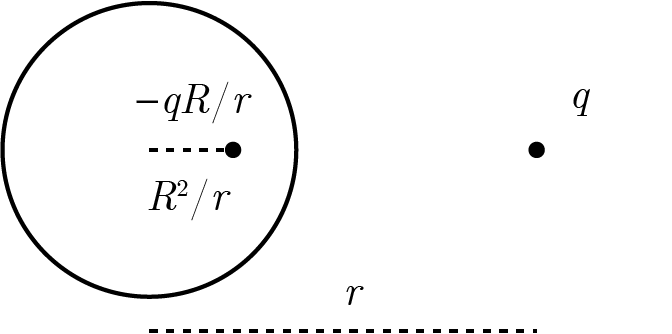
\includegraphics[scale=1]{nall} \end{center}
    \end{itemize}
    Note that these cases correspond to when the conductors are grounded, i.e. their potential is 0.
\end{theorem}

\begin{defn}[Dielectrics]
    For most materials, atoms can rearrange themselves in an electric field to counter the effect of the field. The permittivity of a dielectric is denoted $\epsilon$. The relative permittivity $\kappa$ (sometimes denoted $\epsilon_r$) is given by $\kappa = \epsilon/\epsilon_0.$ The electric field strength is decreased by a factor $\kappa$ within a dielectric; in other words we replace $\epsilon_0$ with $\epsilon$.
\end{defn}

\section{Problem Set}

\subsection{Exercises}

\begin{prob}
    A dipole with moment $p=qd$ is oriented in the $xy$ plane with the charge $+q$ at the point $(0,d/2)$ and the charge $-q$ at the point $(0,-d/2)$. \begin{anum}
        \item Find the potential $\phi(x,y)$ in space as a function of $x$ and $y$ with $x,y\gg d$.
        \item Use your answer from part (a) to find the electric field $\mathbf E(x,y)$ as a function of $x$ and $y$.
    \end{anum}
\end{prob}

\begin{sol}
    \begin{anum}
        \item Using the definition of potential, \begin{align*}\phi(x,y)&=\frac{q}{4\pi\epsilon_0}\left(\frac{1}{\sqrt{x^2+\left(y-\frac d2\right)^2}}-\frac{1}{\sqrt{x^2+\left(y+\frac d2\right)^2}}\right)\\
        &\approx\frac{q}{4\pi\epsilon_0}\left(\frac{1}{\sqrt{x^2+y^2-yd}}-\frac{1}{\sqrt{x^2+y^2+yd}}\right)\\
        &\approx\frac{qdy}{4\pi\epsilon_0(x^2+y^2)^{3/2}}\\
        &\approx \boxed{\frac{py}{4\pi\epsilon_0(x^2+y^2)^{3/2}}}\end{align*}
        \item Taking the derivatives, $$\mathbf{E}(x,y)=\left(-\frac{d\phi}{dx},-\frac{d\phi}{dy}\right)=\boxed{\left(\frac{pxy}{4\pi\epsilon_0(x^2+y^2)^{5/2}},\frac{p(2y^2-x^2)}{4\pi\epsilon_0(x^2+y^2)^{5/2}}\right)}$$
    \end{anum}
\end{sol}

\begin{prob}\label{thing}
    Suppose we have a thin, uniformly charged spherical shell of radius $R$ and total charge $Q$. We will find the electrostatic pressure $P$ on the walls of the shell in two ways.\begin{anum}
        \item First, using only concepts introduced last week (Coulomb's law, electric fields, Gauss's law, etc), find the pressure from evaluating the force acting on a small piece of the shell $dA$.
        \item Now, find the electric potential energy associated with the shell $U$. Now, suppose somehow the radius of the shell increases to $R+dR$ so that the electric potential energy changes by some $dU$. Find this change in energy, and relate it to the work done by the outward electrostatic pressure $P$ when the radius increased by $dR$. Use this equation to then solve for $P$, and verify that it is consistent with your earlier result. This is called the method of virtual work, and is in general a very a useful trick in olympiad physics for finding the magnitude of forces using energy.
    \end{anum}
\end{prob}

\begin{sol}
\begin{anum}
    \item The electric field right outside the sphere is $Q/4\pi\epsilon_0R^2$, and right inside it is 0. Thus the force on a small piece $dA$ is found as $$dF=\frac{Q\, dA}{4\pi R^2}\frac{E_{\text{out}}+E_{\text{in}}}{2}=\frac{Q^2}{32\pi^2 \epsilon_0R^4}dA$$so the pressure is $$P=\frac{dF}{dA}=\boxed{\frac{Q^2}{32\pi^2 \epsilon_0R^4}}$$
    \item In class, we found the potential energy to be $$U=\frac{Q^2}{8\pi \epsilon_0R}$$If the radius increases by $dR$, then we take the derivative to find the corresponding increase in $U$:$$dU=-\frac{Q^2}{8\pi \epsilon_0R^2}dR$$The work done by the pressure if the radius increases by $dR$ is $4\pi R^2P\, dR$, and this equals to $-dU$. as a result, $$4\pi R^2P\, dR=\frac{Q^2}{8\pi \epsilon_0R^2}dR\Rightarrow P=\boxed{\frac{Q^2}{32\pi^2\epsilon_0R^4}}$$which agrees with the result from before.
\end{anum}
\end{sol}

\begin{prob}[Kalda]
    $N$ identical droplets of mercury are charged to the same potential $\phi_0$. Determine the potential of a large drop of mercury when the $N$ smaller droplets coalesce (assume all the droplets are spherical).
\end{prob}

\begin{sol}
    Let the radii of the starting droplets be $r_0$, so that the radius of the final droplet is $r_0\sqrt[3]{N}$. Since the potential is related to the charge $q$ on each droplet as $\phi_0=q/4\pi\epsilon_0r_0$, the total charge is $Nq=4N\phi_0\pi\epsilon_0r_0$. Then the final potential is $$\phi=\frac{4N\phi_0\pi\epsilon_0r_0}{4\pi\epsilon_0r_0\sqrt[3]{N}}=\boxed{\phi_0N^{2/3}}$$
\end{sol}

\begin{prob}
    Two conducting spheres at a very far distance from one another have charge $Q$, but one has radius $r$ and the other has radius $R>r$. The spheres are then connected by a wire (which means they are then forced to have the same potential). After this is done, what is the difference in the charges on the spheres?
\end{prob}

\begin{sol}
    Let $Q_1$ and $Q_2$ be the final charges. Since the spheres are very far from each other, we neglect their electrostatic interaction. The potential on each ball is $\sim q/r$, so after the wire is connected we have $Q_1/R=Q_2/r$. Note also $Q_1+Q_2=2Q$. Solving the system, $$\Delta Q=|Q_1-Q_2|=\boxed{\frac{2Q(R-r)}{R+r}}$$
\end{sol}

\begin{prob}[Purcell]
The shaded regions in the figure below represent two neutral concentric conducting spherical shells. The white regions represent vacuum. Two point charges $q$ are located as shown; the interior one is off-center. \begin{center}
    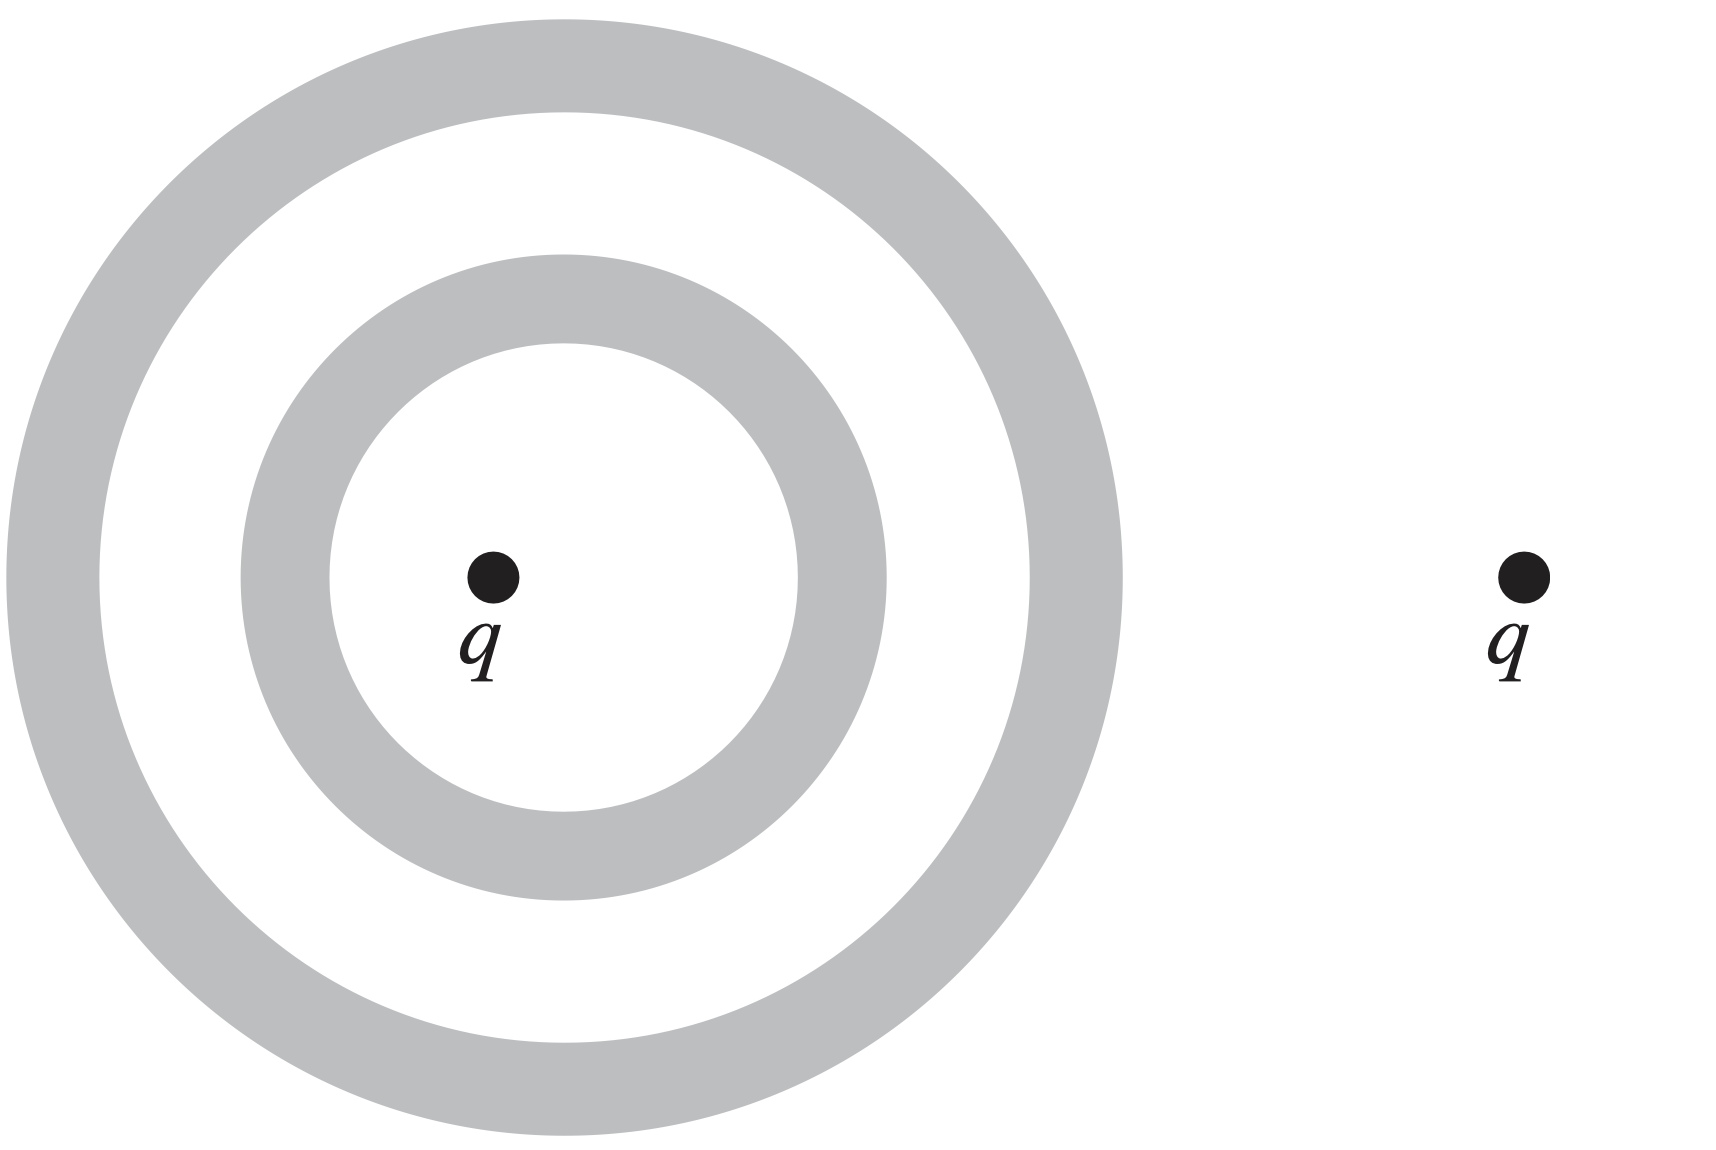
\includegraphics[scale=0.2]{morin3}
\end{center}\begin{anum}
    \item Draw a reasonably accurate picture of the field lines everywhere, and indicate the various charge densities. What quantities are spherically symmetric? (There are two possible cases for what your picture can look like, depending on how close the exterior point charge is. Take your pick.)
    \item Repeat the above tasks in the case where the two shells are connected by a wire, so that they are at the same potential.
\end{anum}
\end{prob}

\begin{sol}
    \begin{anum}
        \item The charge distributions and field lines are shown (roughly) in the figure below.
        \begin{center}
            
\includegraphics[scale=0.25]{sol1.png}
        \end{center} 
        Let the four surfaces be labeled 1, 2, 3, 4, starting from the innermost one. There is charge $-q$ on surface 1. This is true because the field is zero inside the metal of the conductor, so a spherical Gaussian surface drawn inside the metal of the inner conductor has no flux, so the net charge enclosed in the sphere must be zero. The negative surface charge density on surface 1 is higher near the off-center point charge. Since the inner conductor is neutral, a charge $+q$ must reside on surface 2. This surface charge density is spherically symmetric, because it feels no field from the charges inside (or outside) of it, due to the zero field inside the metal of the conductors. By the same Gauss’s-law reasoning, there must be a charge $-q$ on surface 3, because there is zero field inside the metal of the outer conductor. This surface charge density is spherically symmetric. A charge $+q$ is left for surface 4. This surface charge density is actually negative near the outer charge $q$ if that charge is located close enough to the shells. But in any case the total charge on surface 4 is $+q$. Between the shells, the field is spherically symmetric, consistent with the spherically symmetric charge densities on surfaces 2 and 3.
        \item The shells are now at the same potential, so the field between them must be zero. Therefore, the only difference from the scenario in part (a) is that we just need to erase the field between the shells and erase the charges on surfaces 2 and 3. The charges on surfaces 1 and 4 aren’t affected by this change, because the surfaces 2 and 3 together produced zero field everywhere except between them. Basically, when we connect the shells, the charges on surfaces 2 and 3 simply neutralize each other.
    \end{anum}
\end{sol}

\begin{prob}
    Given a point charge $q$ a distance $a$ above an infinite conducting plane, find the surface charge density $\sigma$ on the plane as a function of $r$, the horizontal distance between a point on the plane and the charge $q$. 
\end{prob}

\begin{sol}
    We know that the electric field is equivalent to that generated by an image $-q$ on the other side. Given the magnitude of $E$ at some point on the plane, we can find $\sigma$ via $\sigma = -\epsilon_0E$ (note that $E$ points into the plane, so $\sigma$ is negative). Notice that because of the image, the electric field at the given point is double the vertical component of the charge $q$. We have $$\sigma(r)=-2\epsilon_0E_z=\boxed{-\frac{qa}{2\pi(a^2+r^2)^{3/2}}}$$
\end{sol}

\begin{prob}[Purcell]
    Suppose we have a point charge held a distance $a$ above an infinite conducting plane. If you follow a field line that starts out from the point charge in a horizontal direction, that is, parallel to the plane, where does it meet the surface of the conductor? Hint: Use Gauss's law and your answer to the previous problem.
\end{prob}

\begin{sol}
    We use the Gaussian surface in the following diagram, where a hemisphere is drawn right outside the charge $Q$ and the side of the surface is drawn along the field line. 
    \begin{center}
        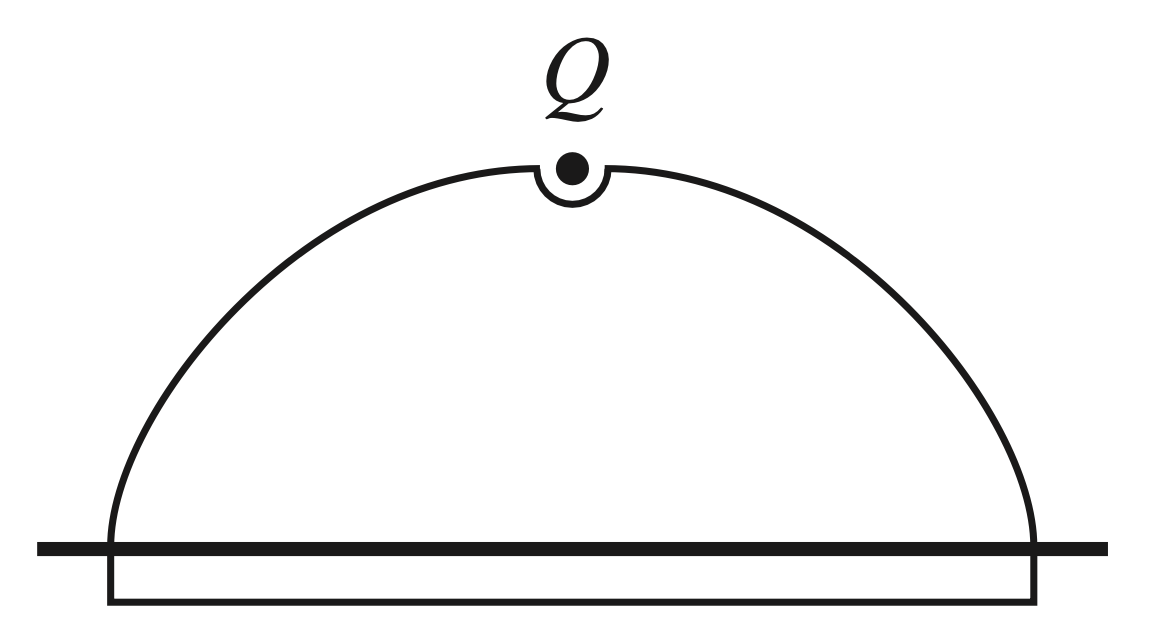
\includegraphics[scale=0.2]{no}
    \end{center}
    The total flux through the surface is equal to the charge enclosed along the plane. Notice that there is no flux out the bottom of the conductor, so the only flux comes from the charge $Q$. The flux into the surface is $Q/2\epsilon_0$, so the total charge enclosed should be $-Q/2$. Using $\sigma$ from earlier, we integrate to the necessary horizontal distance $r$ from the line drawn from $Q$ to the plane until we get $-Q/2$. As a result, $$-\frac{Q}{2}=\int_0^r\sigma (2\pi r)\, dr=\int_0^r -\frac{Qar}{(a^2+r^2)^{3/2}}dr=-Q\left(1-\frac{a}{\sqrt{a^2+r^2}}\right)$$ Thus, $$\frac{a}{\sqrt{a^2+r^2}}=\frac12\Rightarrow r=\boxed{a\sqrt{3}}$$
\end{sol}

\begin{prob}
    A point charge of charge $q$ and mass $m$ is released from rest a distance $a$ above an infinite conducting plane. How long will it take for the charge to collide with the plane? Ignore gravity.
\end{prob}

\begin{sol}
    When the charge is a distance $r$ above the plane, the force on the charge is $q^2/4\pi\epsilon_0(2r)^2$ by the image charge, so its acceleration is $a=q^2/16\pi\epsilon_0mr^2$. We can compare this situation to a gravitational situation. If a mass $m$ is released a distance $a$ from a star, its acceleration at a distance $r$ away is given by $a=GM/r^2$. We can thus compare the two situations with the equivalence $q^2/16\pi\epsilon_0m\equiv GM$. In the gravtiational case, we can easily solve this problem with Kepler's Third law (we covered this problem in Week 13 of the $F=ma$ Course Series). We can take the orbit to be a highly eccentric ellipse of semimajor axis $a/2$, and we take half the period so that $$t=\pi\sqrt{\frac{a^3}{8GM}}=\pi\sqrt{\frac{a^3}{8GM}}\equiv \boxed{\pi\sqrt{\frac{2a^3\pi\epsilon_0m}{q^2}}}$$
\end{sol}

\begin{prob}
    A hollow metal cube has side length $a$. A charge $q$ is placed inside the cube so that it is a distance $d\ll a$ from each of the faces of the cube. Find the force of interaction between the cube and the charge.
\end{prob}

\begin{sol}
    We can assume the faces of the cube to be near infinite planes, so we can build a system of image charges that represents the system. If we consider the image across the bottom face, both the original charge and the image need their own images across one of the side faces, and then those four charges need their images across the last face. The arrangement of charge is thus as shown, with hollow circles representing negative charge: \begin{center}
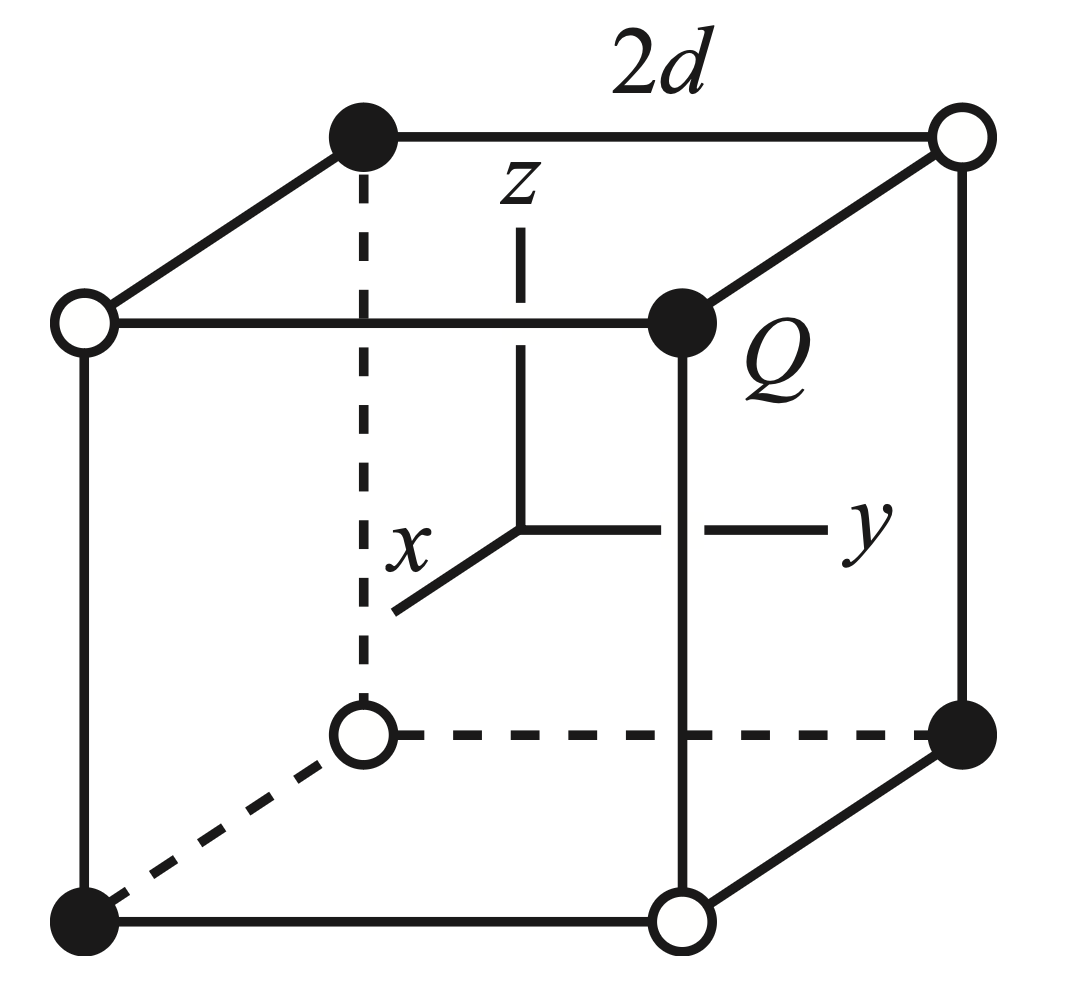
\includegraphics[scale=0.2]{mine}
\end{center}We will consider the contributions of force from the different types of pointss: \begin{itemize}
    \item Three charges $-Q$ at a distance $2d$ make an angle $\cos^{-1}(1/\sqrt 3)$ with the direction toward the origin. This follows from the fact that the diagonal of the cube has length $3(2d)$. We therefore have (ignoring the $4\pi\epsilon_0$), $$F_1=3\frac{Q^2}{(2d)^2}\cdot\frac{1}{\sqrt3}=\frac{\sqrt{3}Q^2}{4d^2}$$This force is directed toward the corner of the cube.
    \item Three charges $Q$ at a distance $2\sqrt 2d$ make an angle $\cos^{-1}(\sqrt2/\sqrt3)$ with the direction toward the origin. So$$F_2=3\frac{Q^2}{(2\sqrt2d)^2}\cdot\frac{\sqrt2}{\sqrt3}=\frac{\sqrt3Q^2}{4\sqrt2d^2}$$This force is directed away from the corner.
    \item One charge $-Q$ at a distance $2\sqrt3d$ is located in line with the origin. So $$F_3=\frac{Q^2}{(2\sqrt3d)^2}=\frac{Q^2}{12d^2}$$This force is directed toward the corner.
\end{itemize}
Adding all the forces together and bringing back the $4\pi\epsilon_0$, we get $$F=\frac{1}{4\pi\epsilon_0}\left(\frac{\sqrt3}{4}-\frac{\sqrt3}{4\sqrt2}+\frac{1}{12}\right)\frac{Q^2}{d^2}\approx \boxed{0.210\frac{Q^2}{4\pi\epsilon_0d^2}}$$
\end{sol}



\begin{prob}
    In this problem we will find the potential energy of a solid ball of uniform charge $Q$ and radius $R$ in two ways.
    \begin{anum}
        \item Integrate the electric field energy density $\epsilon_0E^2/2$ for all points in space.
        \item If we have a ball of charge of radius $r<R$ and charge density equal to the final ball, we can find the work it takes to bring in a thin layer of charge (like a layer of an onion) to cover the ball and increase its radius to $r+dr$. Find the total work necessary to create the entire ball.
    \end{anum}
\end{prob}

\begin{sol}
    \begin{anum}
        \item Inside the ball, $E$ can be found via the shell theorem, so $$E_{\text{in}}=\frac{Q(r^3/R^3)}{4\pi\epsilon_0r^2}=\frac{Qr}{4\pi\epsilon_0R^3}$$Outside, $E$ is simply $$E_{\text{out}}=\frac{Q}{4\pi\epsilon_0r^2}$$So we integrate: $$U=\frac12\epsilon_0\left(\int_0^R\left(\frac{Qr}{4\pi\epsilon_0R^3}\right)^2(4\pi r^2)dr+\int_R^\infty\left(\frac{Q}{4\pi\epsilon_0r^2}\right)^2(4\pi r^2)dr\right)=\boxed{\frac{3Q^2}{20\pi\epsilon_0R}}$$
        \item The potential at the surface of the ball when the radius is $r$ is $\phi=Q(r^3/R^3)/4\pi\epsilon_0r.$ The work $dU$ needed to add in charge to increase the radius by $dr$ is thus $\phi \, dq=\phi Q(4\pi r^2\, dr)/(4\pi R^3/3)$. Integrating, $$U=\int_0^R\frac{Qr^2}{4\pi\epsilon_0R^3}\cdot\frac{Q\cdot4\pi r^2dr}{4\pi R^3/3}=\int_0^R\frac{3Q^2r^4}{4\pi\epsilon_0R^6}dr=\boxed{\frac{3Q^2}{20\pi\epsilon_0R}}$$
    \end{anum}
\end{sol}

\begin{prob}
    A solid sphere of uniform charge $q$ and radius $r$ is surrounded by a spherical, neutral dielectric shell of thickness $t$ and relative resistivity $\kappa$ so that the resulting object is a sphere of radius $R=r+t$. Find the surface charge density $\sigma$ on the surface of the dielectric.
\end{prob}

\begin{sol}
    The electric field at a distance $d$ from the center of the sphere within the dielectric is $E=q/4\pi\kappa \epsilon_0d^2$. Thus by Gauss's law, the charge enclosed is $q/\kappa$, so the charge on the inner surface of the dielectric is $q(1/\kappa)-q.$ The dielectric is neutral, so on the outer surface the charge is the opposite: $q-q(1\kappa)$. We divide by the total area to find $\sigma:$ $$\sigma=\boxed{\frac{q}{4\pi R^2}\left(1-\frac1\kappa\right)}$$
\end{sol}

\subsection{Challenge Problems}

\begin{prob}
    Try Problem 1, Parts 1-4 of APhO 2013 \href{https://apho.olimpicos.net/pdf/APhO_2013_Q1.pdf}{here}.
\end{prob}

\begin{sol}
    See solutions \href{https://apho.olimpicos.net/pdf/APhO_2013_S1.pdf}{here}.
\end{sol}

\begin{prob}[MPPP]
    A solid metal sphere of radius $R$ is divided into two parts by a planar cut, made in such a way that the outer surface of the smaller part of the sphere has surface area $\pi R^2$. The cut surfaces are coated with a negligibly thin insulating layer, and the two parts are put together again so that the original shape of the sphere is restored. Initially the sphere is electrically neutral. 
    \begin{center}
        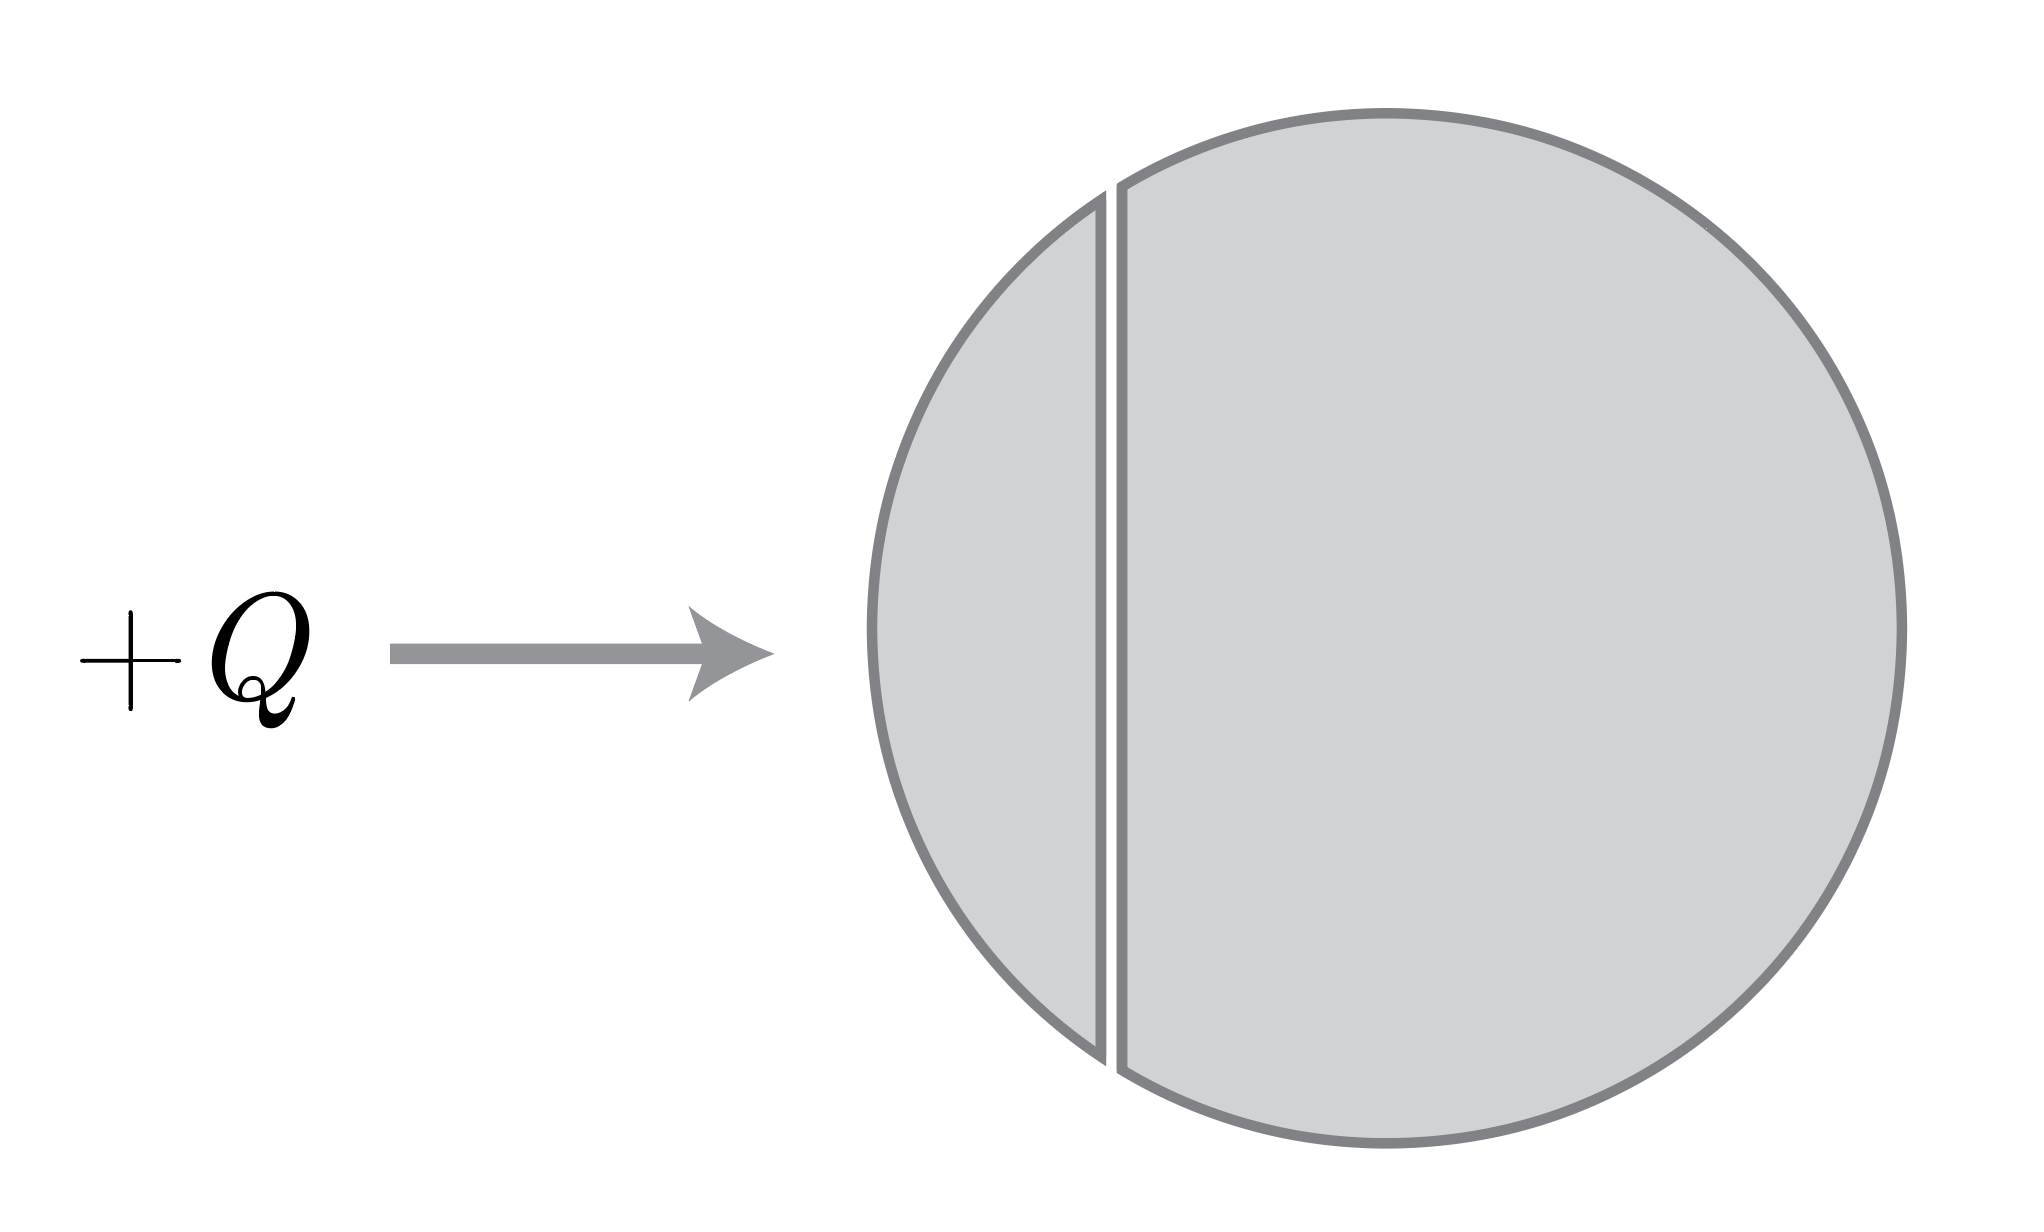
\includegraphics[scale=0.2]{mppp1}
    \end{center}
    The smaller part of the sphere is now given a small positive electric charge $+Q$, while the larger part of the sphere remains neutral. Describe the charge distribution throughout the sphere.
\end{prob}

\begin{sol}
        If we look first at the interface between the two parts, the surface charge densities on the two faces must be exactly opposite one another, because otherwise in the vicinity of those two faces there would exist an electric field within one of the parts of the sphere. Thus, we let two faces carry charges of magnitude $q$. Let $q$ be positive on the left face and negative on the right face, so that the rest of the left part of the sphere has charge $Q-q$ and the rest of the right part of the sphere has charge $q$. Now, when considering the sphere as a whole, note that macroscopically the two charges $\pm q$ on the faces cancel out, so we are just left with a normal conducting sphere. By symmetry, the outer faces of the sphere must therefore have the same charge density. As a result, since the surface area of the left part is $\pi R^2$, we have $$\frac{Q-q}{\pi R^2}=\frac{q}{3\pi R^2}\Rightarrow q=\frac34Q$$
        Thus charge $Q/4$ belongs on the outer surface of the left side with $3Q/4$ on the inner face, while charge $-3Q/4$ lies on the inner face of the right side with $3Q/4$ spread out on its outer surface. 
\end{sol}


\subsection{USAPhO Practice}% Mock?

\begin{prob}[USAPhO 2022 A2]
A droplet of liquid metal has constant mass density and constant surface tension $\sigma$, which causes it to form into a sphere of radius $R$. (Throughout this problem, you may neglect gravity.) A thin wire is inserted into the droplet and connected to an electric current source which slowly increases the charge of the droplet. There is a critical value of the charge, $Q_0$, that causes the droplet to split in half. Each half takes half the total charge, $Q_0/2$, and half the mass of the original droplet. The ``ejected half" is repelled far away from the other half, which remains in contact with the wire.
\begin{anum}
    \item For simplicity, assume the droplet splits as soon as the final state (after the droplet has split in half and the two halves are well separated) has a lower total energy than that of the initial, single droplet. What is the value of $Q_0$? Hint: The energy associated with the surface tension of an object with surface area $S$ is $\sigma S$. Give your answer in terms of a dimensionless constant $A$ multiplied by a product of powers of $\sigma$, $R$, and the vacuum permittivity $\epsilon_0$, and give the numeric value of $A$ to three significant figures.
    \item As more charge is added to the droplet by the current source, it continues to split in half repeatedly. What is the charge $q_n$ on the $n$th ejected droplet? Give your answer in terms of $Q_0$.
    \item In the limit where all of the initial mass of the droplet has been ejected, what is the total work done by the current source? Give your answer in terms of a dimensionless constant $B$ multiplied by a product of powers of $\sigma$, $R$, and $\epsilon_0$, and give the numeric value of $B$ to three significant figures.
\end{anum}
\end{prob}

\begin{sol}
    \officialsol{https://www.aapt.org/physicsteam/upload/2022-USAPhO-solutions.pdf}
\end{sol}

\begin{prob}
    Two large, parallel square conducting plates of side length $s$ are separated by a distance $d\ll s$ and held at this fixed distance by some external force. A dieletric of relative permittivity $\kappa$, mass $m$, and thickness $d$ is placed perfectly in between the plates. Let $x$ reflect the displacement of the dielectric from its initial position. Initially, the charges on the plates are $\pm Q$, and the system is isolated from any other charge. \begin{anum}
        \item Find the surface charge density $\pm \sigma$ on the square faces of the dielectric. 
        \item Find $F(x)$, the electrostatic force acting on the dielectric as a function of $x$. Hint: Use the same virtual work method as in Problem \ref{thing}.
        \begin{center}
            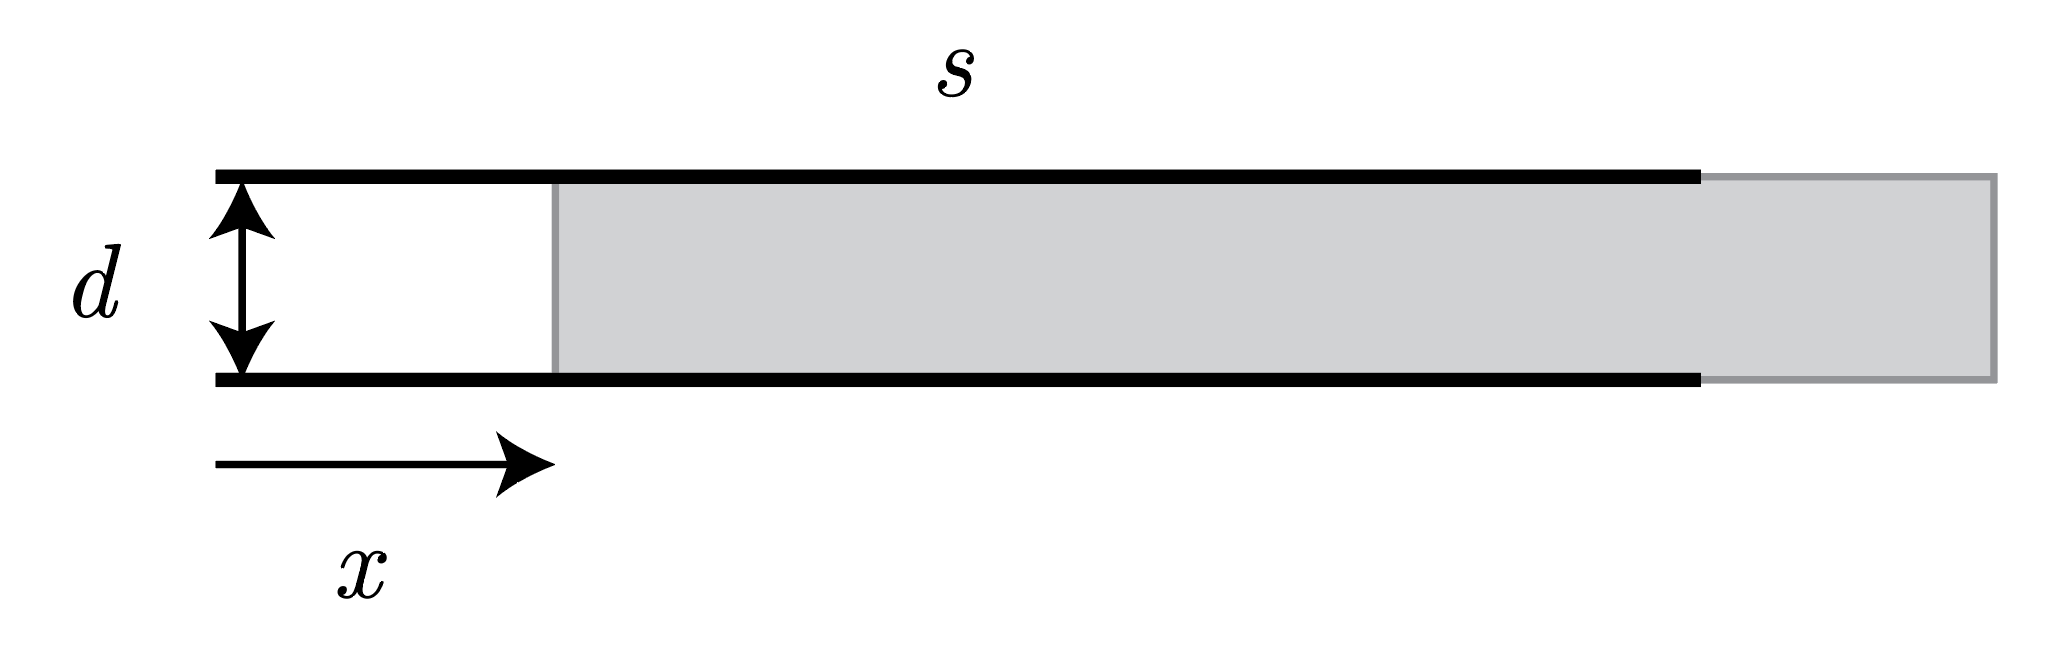
\includegraphics[scale=0.2]{mockusapho2}
        \end{center}
        \item Due to a sharp impulse, the dielectric instantaneously obtains some velocity $v$ parallel to the plates. What is the minimal speed such that the dielectric can escape the gap between the plates?
        \item Now assume that the external force keeping the two plates apart is removed, and in the initial configuration the force keeping the plates apart is due to the dielectric being in the way. Let the dielectric have Young's modulus $Y$. Find the new separation between the plates $d'$.
        %\item Now, find $F(x)$ as defined in part (b), but in the configuration described in part (d). Assume the plates are constrained to be parallel to one another at all times (you can imagine their edges to be attached to rails set a distance $s$ apart). 
        %\begin{center}
            %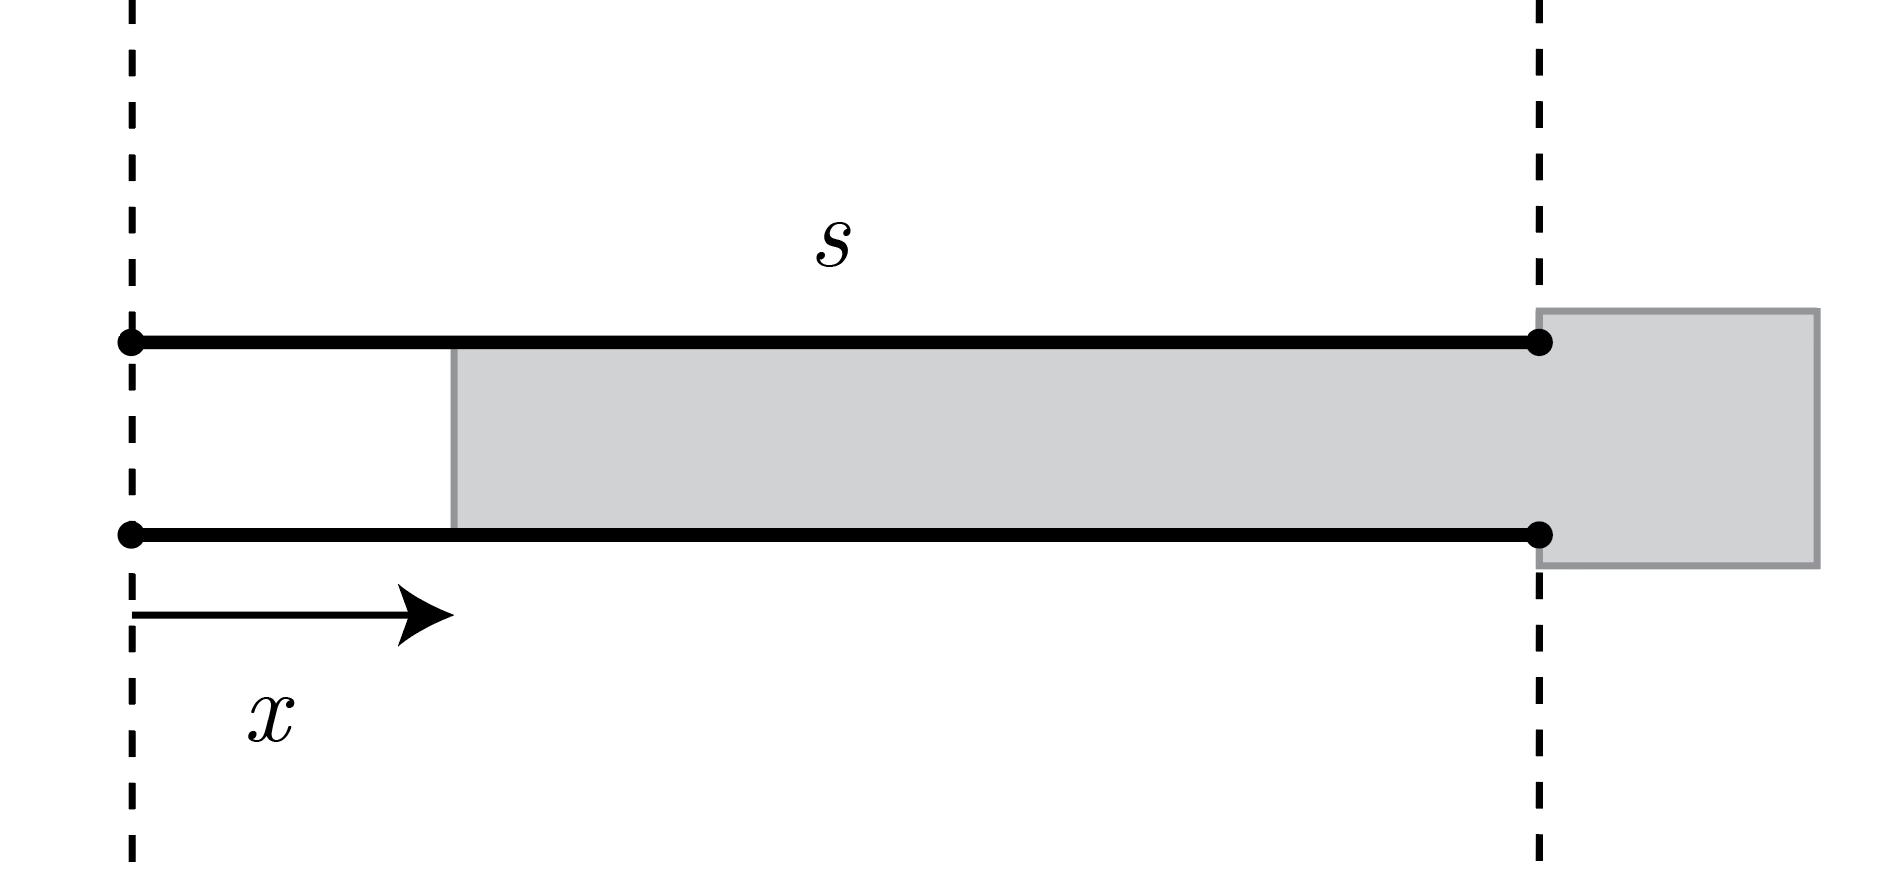
\includegraphics[scale=0.23]{mockusapho3}
        %\end{center}
    \end{anum}
\end{prob}

\begin{sol}
    \begin{anum}
        \item The electric field within the dielectric has magnitude $$E=\frac{Q/s^2}{\epsilon}=\frac{Q}{\kappa \epsilon_0 s^2}$$Thus the net charge on the top and bottom plates (when accounting for the surface charge of the dielectric) is $Q/\kappa$. This means the dielectric surfaces carry charge $Q-Q/\kappa$, so $$\sigma=\boxed{\frac{Q}{s^2}\left(1-\frac1\kappa\right)}$$
        \item Notice that the electric field strength within the vacuum space must equal the electric field strength within the dielectric space, because the conducting plates have constant potential (and must thus have a constant potential difference between them). Let the charge on the plates along the vacuum side be $q$, and that along the dielectric side be $Q-q$. Then, it holds that $$\frac{q}{\epsilon_0x}=\frac{Q-q}{\kappa\epsilon_0(s-x)}\Rightarrow q=\frac{Qx}{\kappa(s-x)+x}$$And so the electric field strength between the plates is $$E=\frac{q}{\epsilon_0sx}=\frac{Q}{\epsilon_0s(\kappa(s-x)+x)}$$
        The energy of the system can be found via integrating the energy density. The energy density is $\epsilon_0E^2/2$ in the vacuum and $\kappa \epsilon_0E^2/2$, so $$U=\frac 12{\epsilon_0 E^2}sxd+\frac 12{\kappa \epsilon_0 E^2}s(s-x)d=\frac{Q^2d}{2\epsilon_0}\frac{1}{s(\kappa(s-x)+x)}$$Taking the derivative, we can find the force as $$F=-\frac{dU}{dx}=\boxed{-\frac{Q^2d(\kappa -1)}{2\epsilon_0s(\kappa s-x(\kappa-1))^2}}$$which is negative, which means the force pulls the dielectric back to the original position. 
        \item The initial energy of the system is equal to the final energy of the system, so $$\frac12mv^2+U(0)=U(s)\Rightarrow \frac12mv^2+\frac{Q^2d}{2\kappa\epsilon_0s^2}=\frac{Q^2d}{2\epsilon_0s^2}\Rightarrow v=\boxed{\sqrt{\frac{Q^2d}{m\epsilon_0s^2}\left(1-\frac1{\kappa }\right)}} $$
        \item Since the force law for the dielectric will follow $F=Ys^2\Delta d/d$, the effective spring constant of the dielectric is $Ys^2/d$. The total energy of the system can thus be described as $$U=\frac{Q^2d'}{2\kappa \epsilon_0s^2}+\frac12\frac{Ys^2}{d}(d-d')^2$$The value of $d'$ in equilibrium is that such that $dU/dd'=0$, so in taking the derivative we get $$\frac{d}{dd'}\left(\frac{Q^2d'}{2\kappa \epsilon_0s^2}+\frac12\frac{Ys^2}{d}(d-d')^2\right)=0\Rightarrow d'=\boxed{d\left(1-\frac{Q^2}{2\kappa\epsilon_0s^4Y}\right)}$$
    \end{anum}
\end{sol}

\end{document}